\documentclass{article}
\usepackage{graphicx} % Required for inserting images
\usepackage{amsmath}
\usepackage{cancel}
\usepackage{enumitem}
\usepackage{geometry}
\usepackage{hyperref}
\usepackage{wrapfig}
\usepackage{comment}
\usepackage{array}
\usepackage{float}
\usepackage{subcaption}
\usepackage{amsmath}
\usepackage{forest}
%\usepackage{table}
\usepackage{xcolor}
\usepackage{tikz}
\usetikzlibrary{shapes, intersections}
\usepackage{multicol}
\usepackage{listings} %for code
\lstdefinestyle{sqlstyle}{
	language=SQL,
	backgroundcolor=\color{lightgray!10},
	basicstyle=\ttfamily\small,
	keywordstyle=\color{blue}\bfseries,
	commentstyle=\color{gray},
	stringstyle=\color{orange!90!black},
	numbers=left,
	numberstyle=\tiny,
	stepnumber=1,
	frame=lines,
	showstringspaces=false,
	tabsize=4,
	breaklines=true
}

\setlength{\parindent}{0pt}
\geometry{
	a4paper,
	total={170mm,257mm},
	left=20mm,
	top=20mm,
}
\title{\Huge \textbf{Basi di dati}
	\small
	
	
	\textit{(aiuto!!!)}}
\author{Matteo Balzerani}
\date{October 2025}

\newcommand{\sitemize}[1]{%
	\begin{itemize}[label=$\diamond$]
		#1
	\end{itemize}
}

\newcommand{\mybox}[1]{%
	\vspace{1em}%
	\noindent\fbox{\colorbox{gray!20}{%
			\begin{minipage}{\dimexpr\textwidth-2\fboxsep}
				#1
			\end{minipage}%
	}}%
	\vspace{1em}%
}

\newcounter{esempio}
\newenvironment{esempio}{
	\refstepcounter{esempio}%
	\noindent\textbf{Esempio \theesempio:}
}{\par}

\graphicspath{{graphics/}}

\begin{document}
	
	\maketitle
	\small
	\begin{multicols}{2}
		\tableofcontents  % <-- Questo genera l'indice
	\end{multicols}
	\newpage
	\normalsize
	\paragraph{Descrizione Esame}
	\begin{itemize}
		\item \textbf{Modulo di Teoria}
		Prova scritta che consiste in domande ed esercizi sugli argomenti trattati. Possibilità di ripetere la prova. In caso di ripetizione della prova, l'ultimo voto ottenuto sostituisce il precedente. 
		
		\item \textbf{Modulo di Laboratorio}
		Prova scritta che consiste in esercizi sugli argomenti trattati. Il voto finale dell'insegnamento di Basi di Dati e Web sarà dato dalla media tra il voto
		della prova scritta di teoria e il voto delle prova scritta di laboratorio. Il voto complessivo verrà pubblicato anche sulla piattaforma MyUnivr e dopo l’accettazione verrà verbalizzato.
	\end{itemize}
	\part{Teoria}
	\section{Introduzione}
	\paragraph{Cos'è un DBMS?} Sistema (prodotto software) in grado di gestire collezioni di dati che siano:
	\begin{itemize}
		\item \textbf{grandi} (di dimensioni (molto) maggiori della memoria centrale dei sistemi di
		calcolo utilizzati). La grandezza richiede che tale gestione sia sofisticata (non
		possiamo caricare tutto in memoria principale e poi
		riscaricare).
		\item \textbf{persistenti} (con un periodo di vita indipendente dalle singole esecuzioni dei
		programmi che le utilizzano). La persistenza richiede una gestione in memoria
		secondaria.
		\item \textbf{condivise} (utilizzate da applicazioni diverse)
			\end{itemize}
		garantendo affidabilità (resistenza a malfunzionamenti
		hardware e software) e privatezza (con una disciplina e un
		controllo degli accessi).
		Come ogni prodotto informatico, un DBMS deve essere
		efficiente (utilizzando al meglio le risorse di spazio e tempo
		del sistema) ed efficace (rendendo produttive le attività dei
		suoi utilizzatori).
		\paragraph{Architettura a livelli dei DBMS}
		I DBMS sono organizzati secondo una architettura a livelli\begin{itemize}
			\item Livello \textbf{LOGICO}: a cui fanno riferimento gli utenti (SQL).
			\item Livello \textbf{FISICO}: stabilisce l’effettiva implementazione in modo efficiente
			
			\textit{Esempio: le relazioni del modello relazionale dei dati vengono realizzate utilizzando varie possibili strutture fisiche}
					\end{itemize} 
			La proprietà di INDIPENDENZA dei dati permette agli utenti di ignorare le strutture fisiche
			– SQL fa riferimento al livello logico
			– Il DBMS si preoccupa di tradurre le operazioni al livello più basso, utilizzando
			in modo efficiente le strutture fisiche. Gli utenti vedono il modello logico (relazionale).
			
			I dati sono in \textbf{memoria secondaria}, le strutture logiche non sarebbe efficienti in memoria secondaria: servono strutture fisiche opportune.
			La memoria secondaria è molto più lenta della memoria principale: serve un'interazione fra memoria principale e secondaria che limiti il più	possibile gli accessi alla secondaria.
			
			\begin{figure}[h!]
				\centering
				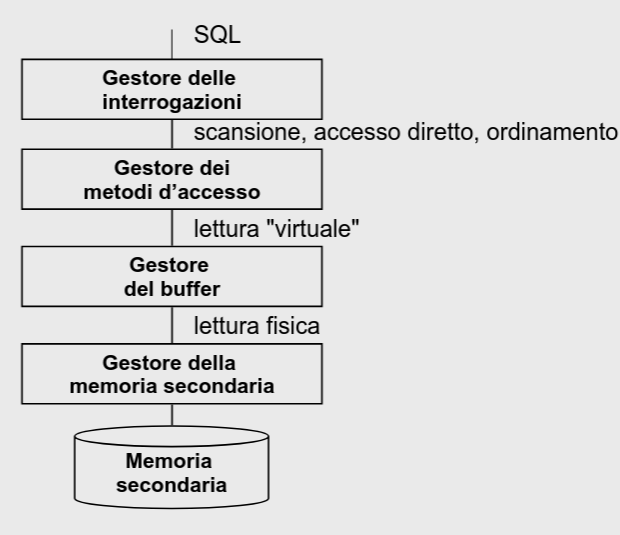
\includegraphics[width=0.4\linewidth]{screenshot001}
				\caption{Architettura della gestione degli accessi e delle interrogazioni in un DBMS}
			\end{figure}
			
			\subsection{Moduli di un DBMS}
			\mybox{\textbf{Domanda d'esame: \textit{Si descrivano i moduli che compongono il DBSM descrivendo brevemente le funzioni di ciascuno:}} risposta nelllo schema sottostante. Bisogna parlare di ciascun modulo brevemente, facendo l'esempio di una query dall'alto verso il basso e viceversa.}
			
			\begin{figure}[h!]
				\centering
				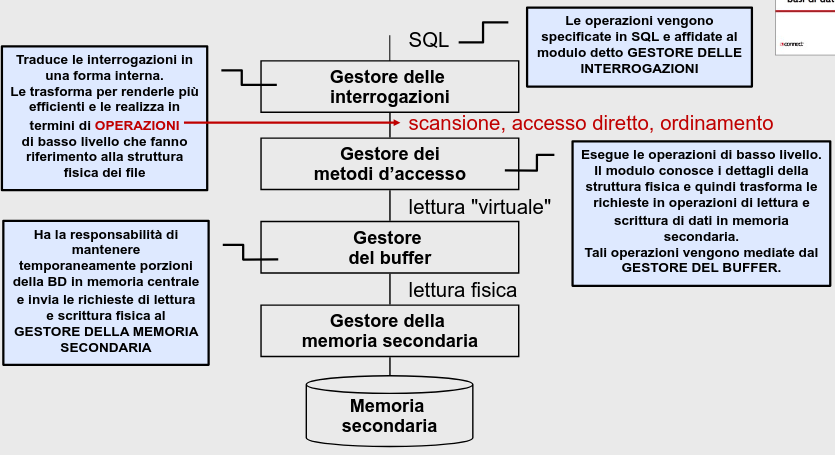
\includegraphics[width=0.7\linewidth]{graphics/screenshot002}
				\caption{}
				\label{fig:screenshot002}
			\end{figure}
			
			\paragraph{Gestore delle interrogazioni} Prende la query logica e la traduce in una forma interna. Le trasforma per renderle più efficienti e le realizza in termini di \textbf{operazioni di basso livello} che fanno riferimento alla struttura fisica dei file.
			
			\paragraph{Gestore dei metodi di accesso} Esegue le operazioni di basso livello. Il modulo conosce i dettagli detta struttura fisica e quindi trasforma le richieste in operazioni di lettura e scrittura di dati in memoria secondaria. Tali operazioni vengono mediate dal GESTORE DEL BUFFER.
			
			\paragraph{Gestore del buffer} Ha la responsabilità di manetenere temporaneamente porzioni della BD in memoria centrale e invia le richieste di lettura e scrittura fisica al \textbf{gestore della memoria secondaria.}
			
			\paragraph{Transazioni} le basi di dati si basano sul concetto di transazione (insieme di operazioni), che deve essere \textbf{atomica}(o tutto o niente) e \textbf{definitiva} (dopo che è andata a buon fine, deve rimanere permanente la transazione eseguita).
			\subsection{Condivisione di una BD}
			Attività diverse su dati in parte condivisi, questo richiede \textbf{meccanismi di autorizzazione} e attività multi-utente su dati condivisi:
			richiedono \textbf{controllo della concorrenza.} L'accesso concorrente in scrittura deve essere regolato.
			
			\begin{figure}[h!]
				\centering
				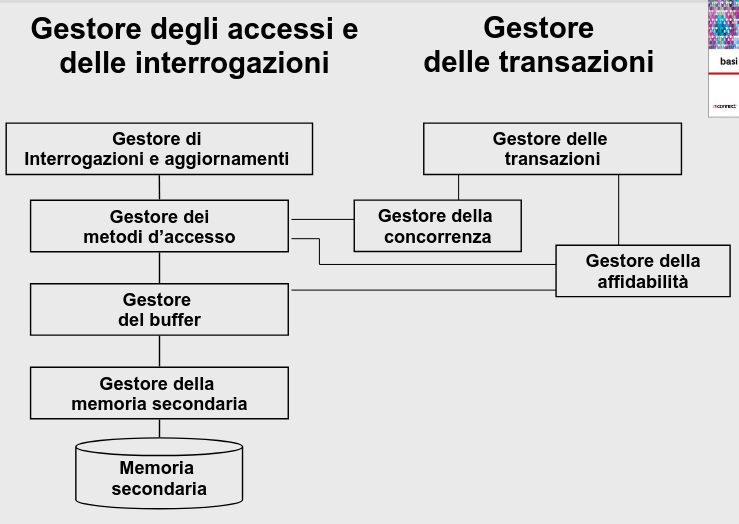
\includegraphics[width=0.4\linewidth]{graphics/screenshot003}
			\end{figure}
			
			Il gestore della concorrenza e il getore della affidabilità sono sottomoduli del gestore delle transazioni (DBMS sistema informativo transazionale.) \textit{Quali sono i moduli che mi permettono di gestire le transazioni in un DBMS?} Significa gestire la concorrenza e gestire l'affidabilità.
			
			\subsection{Gestione della memoria secondaria}
			
			Il costo di un accesso a memoria secondaria è quattro o più ordini di grandezza maggiore di quello per operazioni in memoria centrale. Nelle applicazioni "I/O bound" (cioè con molti accessi a memoria secondaria e relativamente poche operazioni) il
			costo dipende esclusivamente dal numero di accessi a memoria secondaria. Nei DBMS l’interazione tra memoria centrale e secondaria è realizzata attraverso un buffer.
			
			\subsubsection{Buffer}
			\begin{itemize}
				\item Area di memoria centrale, gestita dal DBMS (preallocata) e condivisa fra le
				transazioni.
				\item Organizzato in pagine di dimensioni pari o multiple di quelle dei blocchi di
				memoria secondaria.
				 (Per semplicità ipotizzeremo che ciascuna pagina corrisponda ad un blocco)
				\item L’allocazione di buffer sempre più grandi, riduce il numero di accessi alla
				memoria secondaria
				\item La gestione ottimale del buffer è un aspetto fondamentale nelle BD (rispetto
				alle prestazioni). Il buffer è importantissimo per via della grande differenza di tempo di accesso fra
				memoria centrale e memoria secondaria.
				
			\end{itemize}
			
			\subsubsection{Gestione del buffer}
			\paragraph{Scopo della gestione del buffer}\begin{itemize}
				\item \textbf{Ridurre il numero di accessi alla memoria secondaria}\textit{GARANTENDO L'AFFIDABILITÀ.} \sitemize{\item 
				In caso di \textbf{lettura}, se la pagina è già presente nel buffer, non è necessario
				accedere alla memoria secondaria.
				\item In caso di \textbf{scrittura}, il gestore del buffer può decidere di differire la scrittura
				fisica (ammesso che ciò sia compatibile con la gestione dell’affidabilità)}
				
				\item Le politiche di gestione del buffer assomigliano a quelle
				della gestione della memoria centrale da parte dei Sistemi
				Operativi: obbediscono allo stesso principio, detto di località, in base al quale i dati
				referenziati di recente hanno una maggiore probabilità di essere referenziati
				nuovamente in futuro
			\end{itemize}
			
			Il buffer offre ai moduli di livello più alto una interfaccia complessa, non si limita alle richieste di lettura e scrittura. Ha bisogno delle informazioni sul prevedibile riutilizzo delle pagine (per evitarne la riapertura); Ha bisogno delle informazioni sulla necessità di effettuare immediatamente gli aggiornamenti (per evitare la perdita in caso di guasto). Per la gestione dei buffer sono necessarie le seguenti
			informazioni: \begin{itemize}
				\item Un direttorio che per ogni pagina mantiene (ad esempio) il file fisico e il numero del blocco ad essa corrispondente.
				\item Per ogni pagina del buffer il gestore mantiene due variabili di stato: \textbf{un contatore }che indica quanti programmi utilizzano la pagina e un \textbf{bit} che indica se la pagina è “sporca”, cioè se è stata modificata
			\end{itemize}
		
		\paragraph{Funzioni del buffer manager}
		Le politiche sono simili a quelle relative alla gestione della memoria da parte dei sistemi operativi. 
		
		\mybox{\textbf{Principio di "località dei dati”:} è alta la probabilità di dover riutilizzare i dati attualmente in uso.
		
		\textbf{Legge 80-20:} l'80\% delle operazioni utilizza sempre lo stesso 20\% dei dati.
		}
		
		\paragraph{Operazioni per la gestione del buffer:} \begin{itemize}
			\item \textbf{Fix:} Richiesta di accesso ad una pagina, richiede una lettura solo se la pagina non è nel buffer (incrementa il contatore associato alla pagina), ritorna il riferimento alla pagina nel buffer.
			%%%% SISTEMA %%%
			Cerca la pagina nel buffer: se c'è, restituisce l'indirizzo; per il principio di località ciò avviene abbastanza spesso. Altrimenti, cerca una pagina libera nel buffer (contatore a zero): Se la trova, restituisce l'indirizzo; se il BIT di stato segnala che la pagina è stata modificata, essa viene
			aggiornata in memoria di massa. Altrimenti (se non ci sono pagine libere), due alternative
			– “steal”: selezione di una "vittima", pagina occupata del buffer; i dati della
			vittima sono scritti in memoria secondaria; viene letta la pagina di interesse
			dalla memoria secondaria e si restituisce l'indirizzo
			– “no-steal”: l'operazione viene posta in attesa (che si liberino pagine nel
			buffer)
			
			\item \textbf{setDirty}
			Comunica al buffer manager che la pagina è stata modificata. Viene modificato il BIT di stato relativo.
			\item \textbf{Unfix:} indica che la transazione ha concluso l'utilizzo della pagina, decrementa il contatore associato alla pagina.
			\item \textbf{Force:} Trasferisce in modo sincrono una pagina in memoria secondaria \textbf{su richiesta del gestore dell'affidabilità} (non del gestore degli accessi) per garantire che alcuni dati non vengano persi. Memorizza in maniera permanente le modifiche per garantire l'affidabilità.
		\end{itemize}
	
		\mybox{La scrittura in memoria secondaria può avvenire in due
			modi: \begin{itemize}
				\item in modo sincrono quando è richiesto esplicitamente con una force
				\item in modo asincrono (indipendente dall’applicazione) quando il buffer
				manager lo ritiene opportuno (o necessario). In particolare, può decidere di anticipare o posticipare scritture per coordinarle
				e/o sfruttare la disponibilità dei dispositivi
			\end{itemize}
		}
			
			
			
			
			
			
			
			
			
			
			
			
			
			
			
			
			
			
			
			
			
			
			
			
			
			
			
			
			
			
			
			
			
			
			
			
			
			
			
			\newpage
			\section{Possibili domande d'esame}
			\begin{itemize}
				\item \textbf{\textit{Si descrivano i moduli che compongono il DBSM descrivendo brevemente le funzioni di ciascuno:}} risposta nelllo schema sottostante.
				
				\begin{figure}[h!]
					\centering
					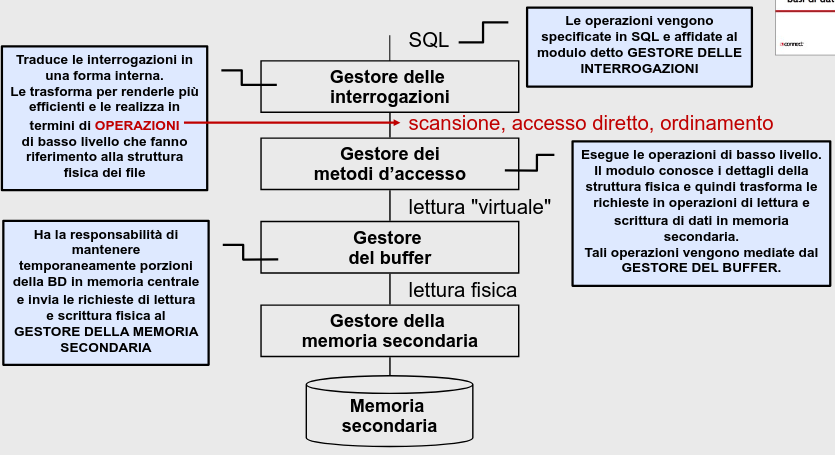
\includegraphics[width=0.7\linewidth]{graphics/screenshot002}
				\end{figure}
				
				Bisogna parlare di ciascun modulo brevemente, facendo l'esempio di una query dall'alto verso il basso e viceversa.
				
				\item \textbf{\textit{(da approfondire) Quali sono i moduli che mi permettono di gestire le transazioni in un DBMS?}} Significa gestire la concorrenza e gestire l'affidabilità.
				
					\begin{figure}[h!]
					\centering
					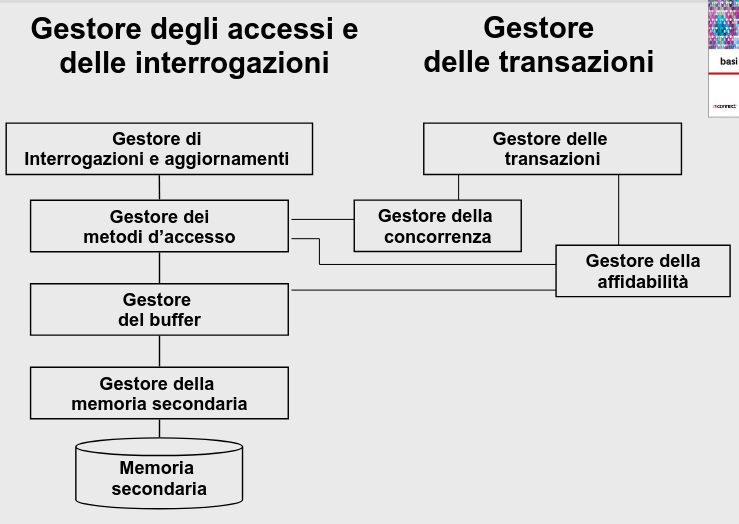
\includegraphics[width=0.7\linewidth]{graphics/screenshot003}
				\end{figure}
				
				\item \textit{\textbf{Si descriva in che modo le tuple vengono organizzate nelle pagine:}} 
			\end{itemize}
\end{document} 